\documentclass[a4paper]{article}

%%% packages %%%%%%%%%%%%%%%%%%%%%%%%%%%%%%%%%%%%%%%%%%%%%%%%%%%%%%%%%%%%%%%%%
\usepackage{graphicx}
\usepackage{amsmath,amssymb}
\usepackage{alltt}
\usepackage{natbib} % please use \citep and \citet instead of \cite

\usepackage{hyperref}
\usepackage{xcolor}
\definecolor{dark-red}{rgb}{0.4,0.15,0.15}
\definecolor{dark-blue}{rgb}{0.15,0.15,0.8}
\definecolor{medium-blue}{rgb}{0,0,0.5}
\hypersetup{
	colorlinks, linkcolor={dark-red},
	citecolor={dark-blue}, urlcolor={medium-blue}
}

\graphicspath{{./figs/}}
\DeclareGraphicsExtensions{.pdf}

\setlength{\parindent}{0mm}

\usepackage{fancyhdr}

%%% %%%%%%%%%%%%%%%%%%%%%%%%%%%%%%%%%%%%%%%%%%%%%%%%%%%%%%%%%%%%%%%%%%%%%%%%%

\makeatletter
\newcommand{\seminar}{Seminar Cyber-Physical Systems (WS 2019/20)}
\title{\textbf{Prioritized Sweeping Neural DynaQ:\\ Boost Learning by Dreaming}}\let\Title\@title
\newcommand{\sTitle}{Prioritized Sweeping Neural DynaQ}
\newcommand{\AuthorName}{Alexander Osiik}
\author{\AuthorName\\
	\href{mailto:alexander.osiik@student.uni-luebeck.de}{alexander.osiik@student.uni-luebeck.de}\\
	\small \seminar\\
%	\small Service Robotics Group\\
	\small Institute of Computer Engineering, University of L\"ubeck\\
}\let\Author\@author
\makeatother

\pagestyle{fancy}
\renewcommand{\footrulewidth}{0.4pt}
\lfoot{\seminar}
\cfoot{}
\rfoot{\thepage}
\lhead{\AuthorName}
\rhead{\sTitle}

%%% %%%%%%%%%%%%%%%%%%%%%%%%%%%%%%%%%%%%%%%%%%%%%%%%%%%%%%%%%%%%%%%%%%%%%%%%%

\begin{document}
	\maketitle
	
	\begin{abstract}
		\noindent%
		Hier beschreiben welche Hintergründe und Analogien aus der Biologie Reinforcement Learning hat.\\
		State of the Art.\\
		Was Zielsetzung im Original-Paper war, wie sie erreicht wurde und wie es im Projekt umgesetzt wurde.
	\end{abstract}
	
	
	\section{Introduction}
	\label{sec:introduction}
%	Swarm robotics~\citep{brambilla13} bla bla bla.
%	\citet{hamann18} describes bla bla bla
%	see Sec.~\ref{sec:results}
	\begin{itemize}
		\item Hier beschreiben welche Hintergründe und Analogien aus der Biologie Reinforcement Learning hat
		\item State of the Art, medizinische Aspekte, Forschungshintergründe
		\item Was Zielsetzung im Original-Paper, Übertragen der \textbf{hippocambal replays} auf RL.\\
		``... replay refers to the re-occurrence of a sequence of cell activations that also occurred during activity, but the replay has a much faster time scale.''
		\item Aufbau des Experiments
	\end{itemize}


	\section{Reinforcement Learning}
%	\label{sec:rl}
%	see Fig.~\ref{fig:image}	

	\subsection{Markov Decision Problem}
	A Markov Decision Problem (MDP) is a model for problems, where an agent tries to interact with the environment in such way that the utmost reward is achieved. Specifically, the robot is moving (\textit{transition}) through various \textit{states}, having chosen a specific \textit{action} in each state. Each \textit{reward} is determined by initial state, the action and the following state. 
	All transitions are not deterministic, but rather probabilistic, where each probability only depends on the current state and the current action, see \textbf{Markov Assumption}. That way there has to be one initial state, but multiple end states are possible.\\
	The main goal is to find a reward maximizing \textbf{policiy}, by which the agent selects actions where the maximum reward can be expected.\\
	\begin{itemize}
		\item $S:$ Set of states $\{s_1,s_2,\dots, s_n\}$
		\item $A:$ Set of actions $\{a_1,a_2,\dots, a_n\}$ 
		\item $T: S\times A \times S: $ Transition function, which is the probability of going from state $s$ to state $s'$ via action $a$
		\item $R: S\times A \times S \rightarrow \mathbb{R}: $ Reward function
		\item $\Pi:$ Policy, where an optimal action is assigned to each state
		\item $\gamma \in [0,1]$ Discount factor. This factor determines the degree of exploration for the agent. For $\gamma=0$, the agent will stick to the policy, and explot the current (possibly) optimal policy. For $\gamma=1$, the agent will take into account the next states reward, leading to exploration behaviour. A value <1 is a contraint, which limits the maximal obtainable reward, leading to a reduction of cycles.
	\end{itemize}
	The \textbf{V-Values} and \textbf{Q-Values} are certain grading schemes used to solve MDPs. It is the total reward the agent can expect, if it performs the optimal, or maximally benefitting, action $a$ in state $s$, and continues to act optimally.
	\begin{equation}\label{eq:vvalue}
		V^*(s) = \max_{a \in A} \sum_{s' \in S}^{} T(s,a,s')[R(s,a,s')+\gamma V^*(s')]
	\end{equation}
	As the values from equation \ref{eq:vvalue} is hard do compute, a technique called \textbf{Value Iteration} is used. It is used do discretize the equation: 
	\begin{equation}\label{eq:value-iteration}
		V^*(s) = \max_{a \in A} \sum_{s' \in S}^{} T(s,a,s')[R(s,a,s')+\gamma V^*(s')]
	\end{equation}
	where $k$ is the radius from the goal state to the agent. For example, regarding the manhattan norm in a 2D plane, the amount of steps the agent has left until it reaches an end state.\\
	After that, \textbf{Policy Extraction} is performed. It is the assignment of an action to each state, maximizing the expected total reward.
	\begin{equation}
		\Pi^*(s) = \text{arg}\max_{a \in A} \sum_{s' \in S}^{} T(s,a,s')[R(s,a,s')+\gamma V^*(s')]
	\end{equation}
	\begin{itemize}
		\item Einführung \textbf{Markov Decision Problem}
		\item Erklärung der Notation für \textit{state}, \textit{action}, \textit{transition function}, \textit{learning rate}, \textit{discount factor}
		\item Unterschiede \textit{value iteration}, \textit{policy extraction}, \textit{prioritized sweeping}
		\item spätestens hier müsste die Bellman Gleichung stehen:
		
		\item Erklärung Q-Learning, Vorteile, Nachteile
		$$Q(s,a) \leftarrow Q(s,a) + \alpha[r + \gamma \max_{a' \in A}Q(s',a')-Q(s,a)]$$
		\item Exploration/Exploitation TradeOff und Techniken
		\item \textbf{HIER:} Idee des Papers: künstliche Erweiterung des State space umd RL für vergangenheitsabhängige Probleme anwendbar zu machen.
	\end{itemize}
	
	
	\section{GALMO}
	\label{sec:galmo}
	\begin{itemize}
		\item Vorstellung der Ergebnisse des Original Paper (GALMO)
	\end{itemize}
	
	
	\section{Project}
	\label{sec:project}
	\begin{itemize}
		\item Umsetzung von Q-Learning in Python
		\item DQN
		\item Implementierung GALMO?
	\end{itemize}
	
	
	\section{Results}
	\label{sec:results}
	
	
	\begin{figure}[t]
		\centering
		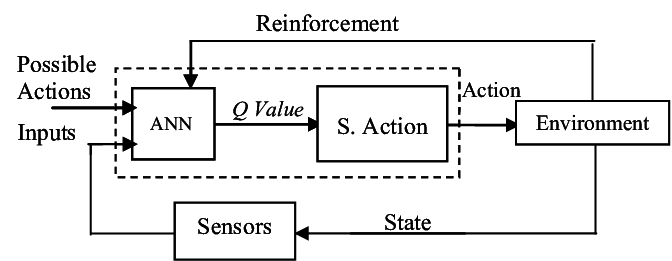
\includegraphics[angle=0,width=0.7\textwidth]{./figs/RL_ANN.png}
		\caption{\label{fig:image}Basic Q-Learning.}
	\end{figure}
	
	
	
	\section{Conclusion}
	
	
	\footnotesize
	\bibliographystyle{plainnat}
	\bibliography{./main}
	
\end{document}
